\documentclass[a4paper, 12pt]{article}

\usepackage{graphicx}
\usepackage{longtable}
\graphicspath{ {images/} }

\newcommand{\templates}{../../template}
\usepackage[a4paper, margin=2.5cm]{geometry}

\usepackage{enumitem}
\setlist[itemize]{noitemsep}
\setlist[enumerate]{noitemsep}

\let\oldpar\paragraph
\renewcommand{\paragraph}[1]{\oldpar{#1\\}\noindent}
\usepackage{graphicx}
\usepackage{hyperref}
\usepackage{makecell}

\newcommand{\settitolo}[1]{\newcommand{\titolo}{#1\\}}
\newcommand{\setprogetto}[1]{\newcommand{\progetto}{#1\\}}
\newcommand{\setcommittenti}[1]{\newcommand{\committenti}{#1\\}}
\newcommand{\setredattori}[1]{\newcommand{\redattori}{#1\\}}
\newcommand{\setrevisori}[1]{\newcommand{\revisori}{#1\\}}
\newcommand{\setresponsabili}[1]{\newcommand{\responsabili}{#1\\}}
\newcommand{\setversione}[1]{
	\ifdefined\versione\renewcommand{\versione}{#1\\}
	\else\newcommand{\versione}{#1\\}\fi
}
\newcommand{\setdestuso}[1]{\newcommand{\uso}{#1\\}}
\newcommand{\setdescrizione}[1]{\newcommand{\descrizione}{#1\\}}

\newcommand{\makefrontpage}{
	\begin{titlepage}
		\begin{center}

		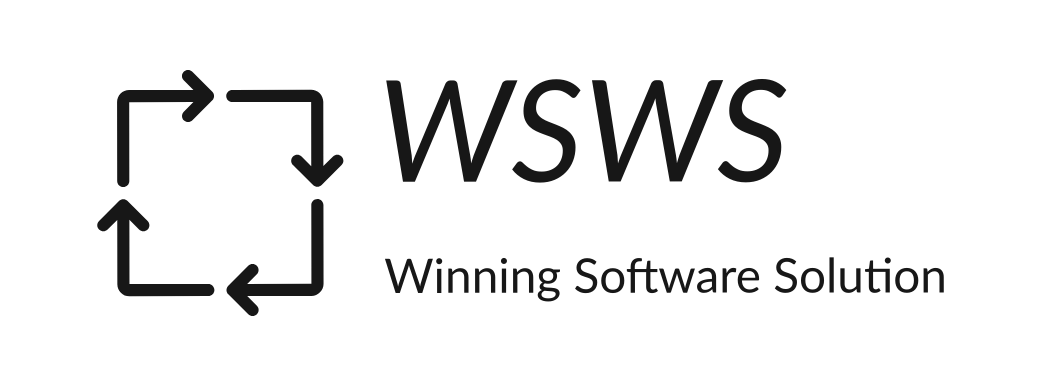
\includegraphics[width=0.4\textwidth]{../../template/WSWS-logos_transparent_crop}\\

		{\Large Winning Software Solution}\\[6pt]
		\href{mailto://winningsoftwaresolution@gmail.com}{winningsoftwaresolution@gmail.com}\\
		
		\ifdefined\progetto
		\vspace{1cm}
		{\Large\progetto}
		{\large\committenti}
		\else\fi
		
		\vspace{1.5cm}
		{\LARGE\titolo}
		
		\vfill
		
		\begin{tabular}{r | l}
		\multicolumn{2}{c}{\textit{Informazioni}}\\
		\hline
		
		\ifdefined\redattori
			\textit{Redattori} &
			\makecell[l]{\redattori}\\
		\else\fi
		\ifdefined\revisori
			\textit{Revisori} &
			\makecell[l]{\revisori}\\
		\else\fi
		\ifdefined\responsabili
			\textit{Respondabili} &
			\makecell[l]{\responsabili}\\
		\else\fi
		
		\ifdefined\versione
			\textit{Versione} & \versione
		\else\fi
		
		\textit{Uso} & \uso
		
		\end{tabular}
		
		\vspace{2cm}
		
		\ifdefined\descrizione
		Descrizione
		\vspace{6pt}
		\hrule
		\descrizione
		\else\fi
		\end{center}
	\end{titlepage}
}
\usepackage{hyperref}
\usepackage{array}
\usepackage{tabularx}

\def\vers#1-#2-#3-#4-#5\\{#1&#2&#3&#4&#5\\\hline}

\newcommand{\addversione}[5]{
	\ifdefined\versioni
		\let\old\versioni
		\renewcommand{\versioni}{#1&#2&#3&#4&#5\\\hline\old}
	\else
		\newcommand{\versioni}{#1&#2&#3&#4&#5\\\hline}
	\fi
}

\newcommand{\setversioni}[1]{\newcommand{\versioni}{#1}}

\newcommand{\makeversioni}{
	\begin{center}
		\begin{tabularx}{\textwidth}{|c|c|c|c|X|}
		\hline
		\textbf{Versione} & \textbf{Data} & \textbf{Persona} & \textbf{Attivtà} & \textbf{Descrizione} \\
		\hline
		\versioni
		\end{tabularx}
	\end{center}
	\clearpage
}

\settitolo{Analisi dei requisiti}
\setprogetto{ShopChain}
\setcommittenti{SyncLab}
\setredattori{Giovanni Cocco}
\setrevisori{Federico Marchi}
\setresponsabili{Giovanni Cocco}
\setdestuso{esterno}
\setdescrizione{
Architettura del progetto
}

\addversione{0.0.0}{23/2/2022}{Giovanni Cocco}{Redazione}{Strutturazione del documento}

\begin{document}

\makefrontpage

\makeversioni

\section{Introduzone}
\subsection{Scopo del documento}
Il documento illustra le scelte architetturali e illustra l'architettura tramite diagrammi delle classi e di sequenza.

\section{Architettura generale}
Il progetto si compone di 4 macro parti:
\begin{itemize}
\item Server
\item Smart contract
\item Web app
\item Script di messa in vendita
\end{itemize}
\subsection{Server}
Realizzato in typescript con express come modulo http e MariaDB come database SQL.
Si divide in 2 parti principali: la persistenza e il server web.
\subsubsection{Persistenza}
Si occupa di gestire i dati delle transazioni.\\\\
Si collega allo smart contract attraverso un websocket fornito da moralis.io.\\
Rimane in ascolto degli eventi dello smart contract e 
aggiorna il database SQL di conseguenza.\\
Tiene sempre traccia dell'ultimo blocco da cui ha ricevuto un evento
e all'avvio recupera tutti gli eventi arretrati partendo da quest'ultimo blocco.\\\\
I dati nel database SQL vengono forniti al frontend.\\\\
Notare come è molto oneroso
effettuare query sui dati in block chain in quanto non sono disponibili strutture dati adeguate.\\
Questa soluzione ci permette una maggiore flessibilità e apertura a modifiche future quali aggiungere query specifiche.\\\\
Inoltre il contratto una volta publicato non può essere modificabile al fine di garantire la trasparenza ed è quindi cruciale
che il codice di quest'ultimo sia semplice ed affidabile.
\subsubsection{Server Web}
Riceve le richieste HTTP dalla rete e risponde con le pagine della Web app.

\subsection{Smart contract}
Realizzato in solidity e publicato su una rete Polygon tiene traccia delle transazioni; gestisce la logica e la sicurezza di esse.\\\\
Per gestire il timer che fa scadere le transazioni si usa il servizio Upkeeper di ChainLink.\\
Uno smart contract non esegue operazioni se non viene chiamato, per realizzare un timer si realizzano delle funzioni che se è passato abbastanza tempo
eseguono le operazioni. Upkeeper chiama automaticamente queste funzioni dall'esterno a intervalli di tempo prefissato.

\subsection{Web app}
Fornita all'utente tramite il server web fornisce la logica lato client.\\
Tramite MetaMask l'utente interagisce direttamente col contratto.\\\\
In caso di utenti mobile reindirizza tramite DeepLink per aprire la pagine sull'app di Metamask.\\\\
I deep link vengono usati anche per il QR code di ricezione del pacco.\\
Possono essere scansionati sia da dentro l'app di MetaMask che dalla fotocamera del cellulare.

\subsection{Script di messa in vendita}
Usato dall'ecommerce per inserire prodotti in vendita in blockchain al fine di verificare che il prezzo sia corretto al momento della vendita.
Realizzato in python per flessibilità, si connette alla block chain tramite moralis.io.
\clearpage

\section{Design pattern}
Nonostante le tecnologie esoteriche del capitolato non si prestino a molti design pattern ne sono stati comunque utilizzati diversi.
\subsection{Constructor injection}
Molto usato nell'architettura del server permette di tener traccia delle dipendenze e rende più facile la realizzazione dei mock per i test di unità
\subsection{Builder}
La creazione del server è molto articolata. Richieda sia la classe Sever che la classe ShopContractEventManger. Queste due classi hanno alcuni argomenti di
costruzione comuni.\\
Per semplificare la costruzione e assicurare che sia tutto configurato la classe ServerManager si comporta come un builder. L'unica differenze è che al posto
di un metodo build v'è il metodo start.
\subsection{Singleton}
L'utilizzo del pattern del singleton è stata inizialmente presa in considerazione, ma poi scartata in quanto complicava la fase di testing e mocking.
\section{Diagramma delle classi}
Notare che in solidity i metodi e le funzioni possono avere come visibilità \textbf{external}. Non essendo disponibile nello standard UML si userà la notazione \textbf{\~} per indicarla.\\\\
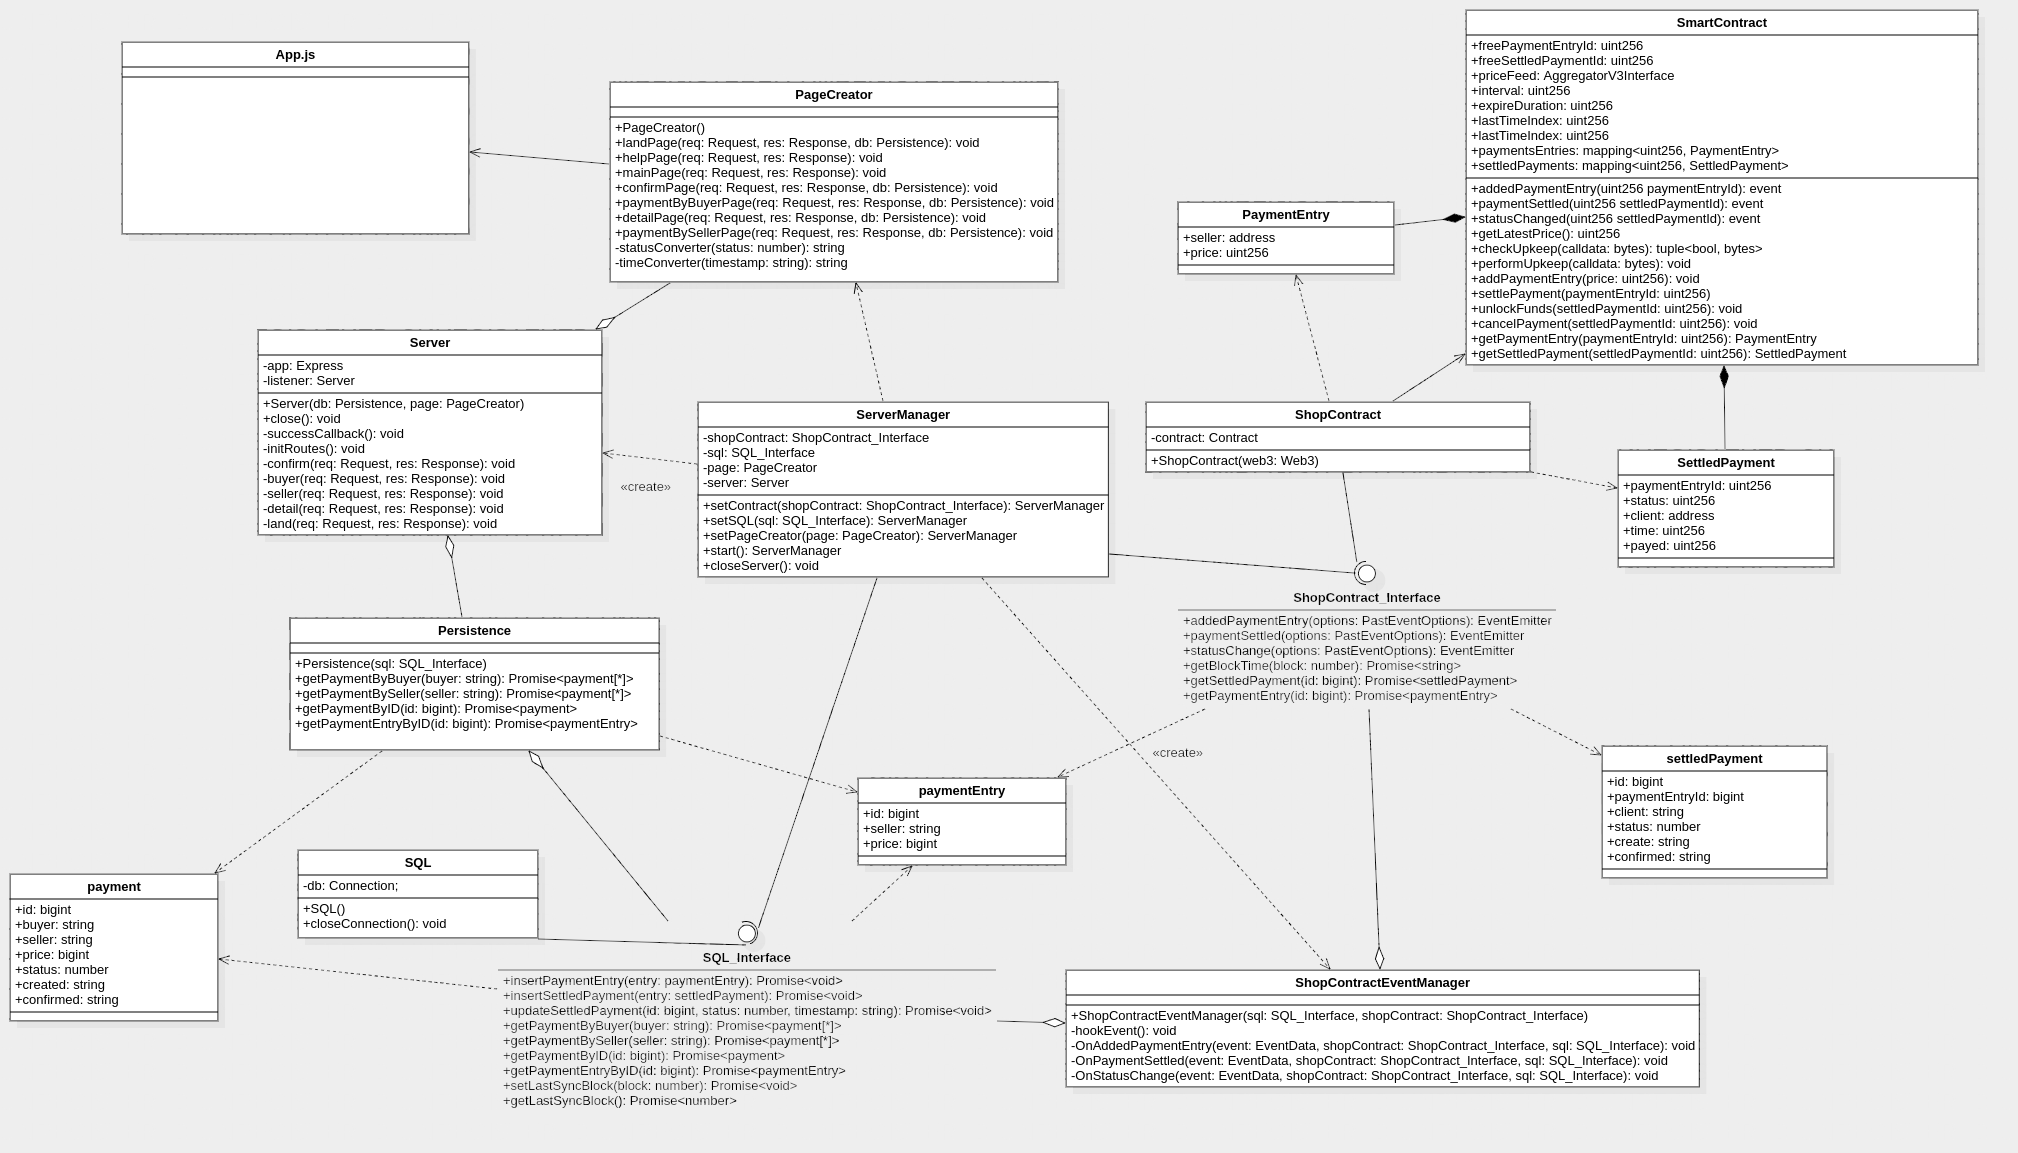
\includegraphics[width=1.0\textwidth]{classes}
\clearpage
\section{Diagrammi di sequenza}
\paragraph{Avvio server}\\
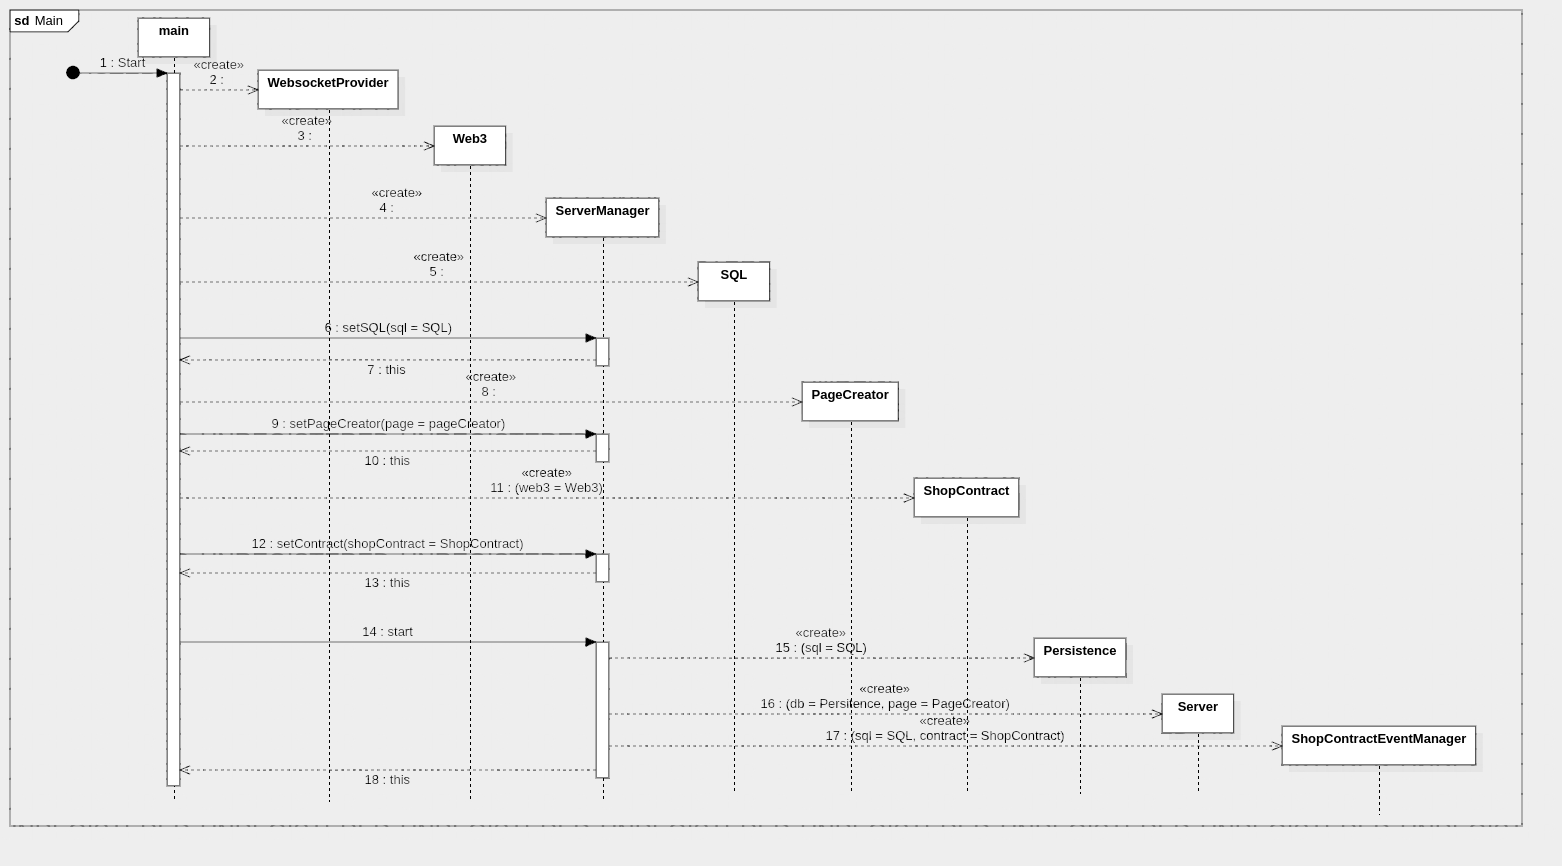
\includegraphics[width=1.0\textwidth]{main}

\paragraph{Ascolto eventi del contratto}\\
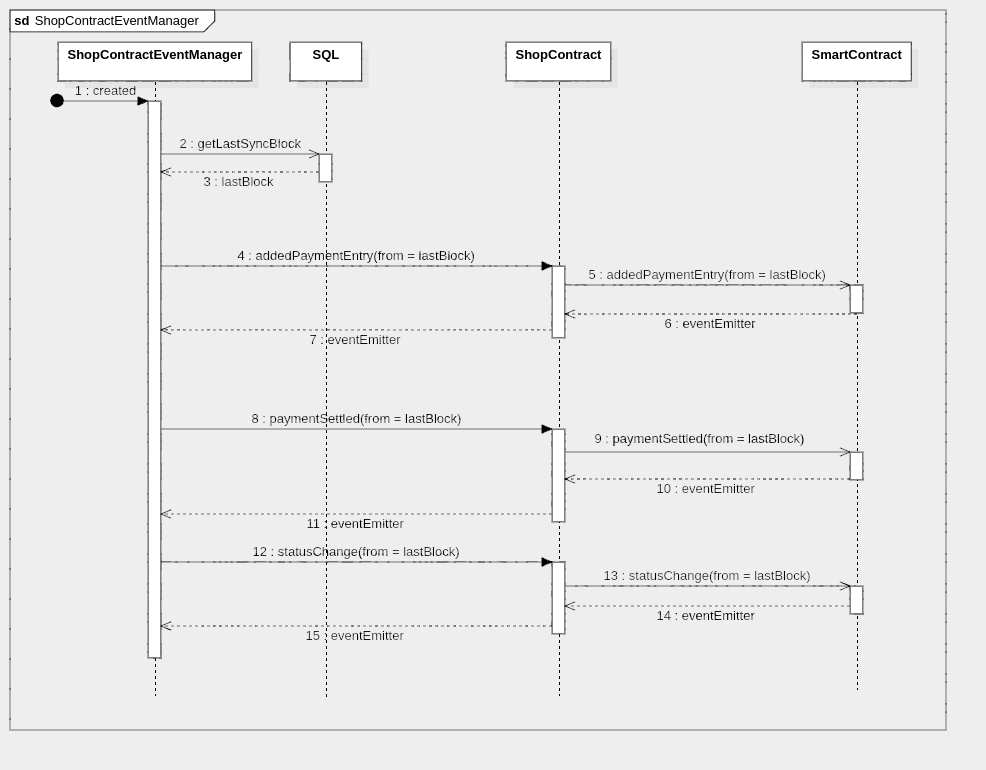
\includegraphics[width=0.9\textwidth]{event}

\paragraph{Inizializzazione server web}\\
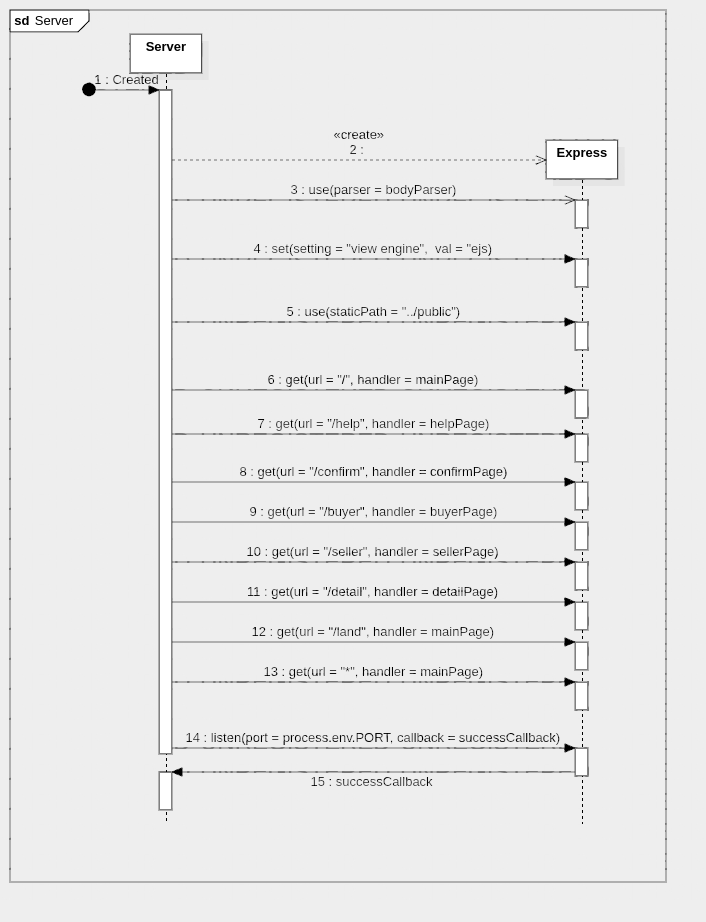
\includegraphics[width=1.0\textwidth]{server}
\clearpage
\paragraph{Nuovo oggetto in vendita}\\
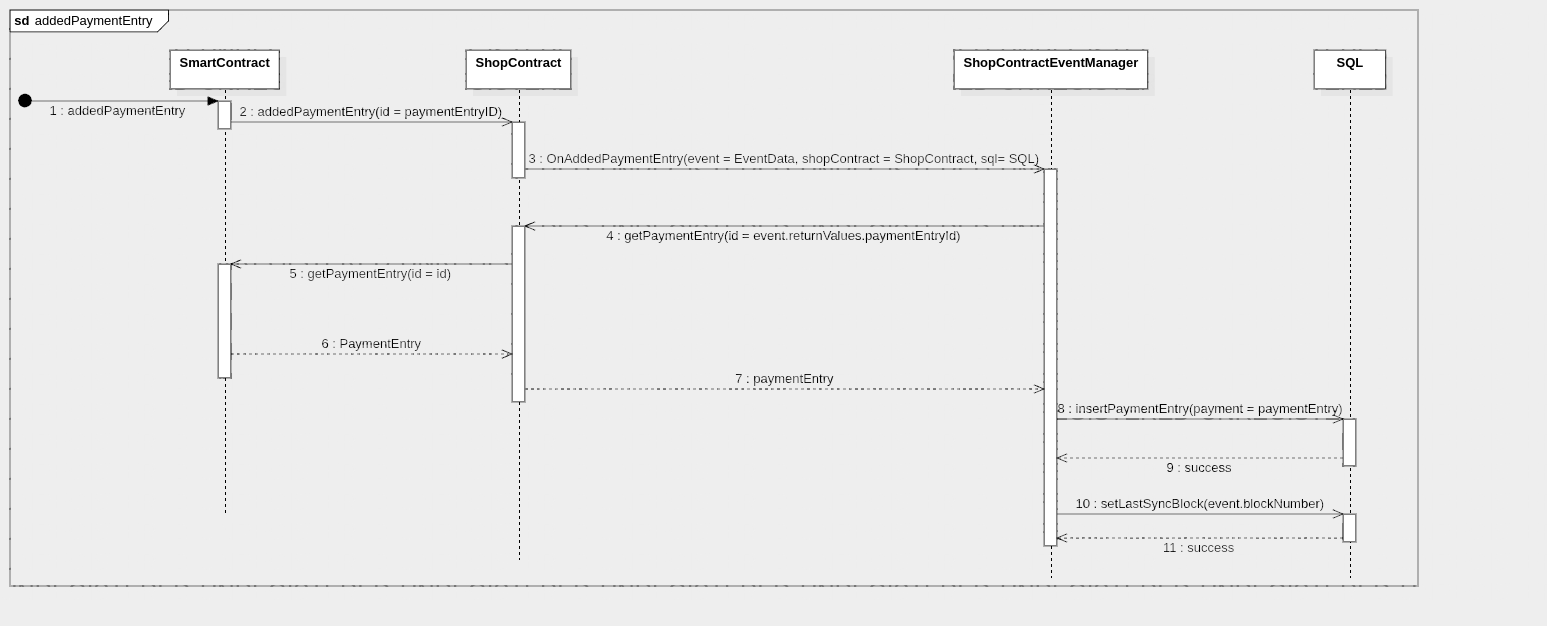
\includegraphics[width=0.85\textwidth]{entry}

\paragraph{Nuova transazione}\\
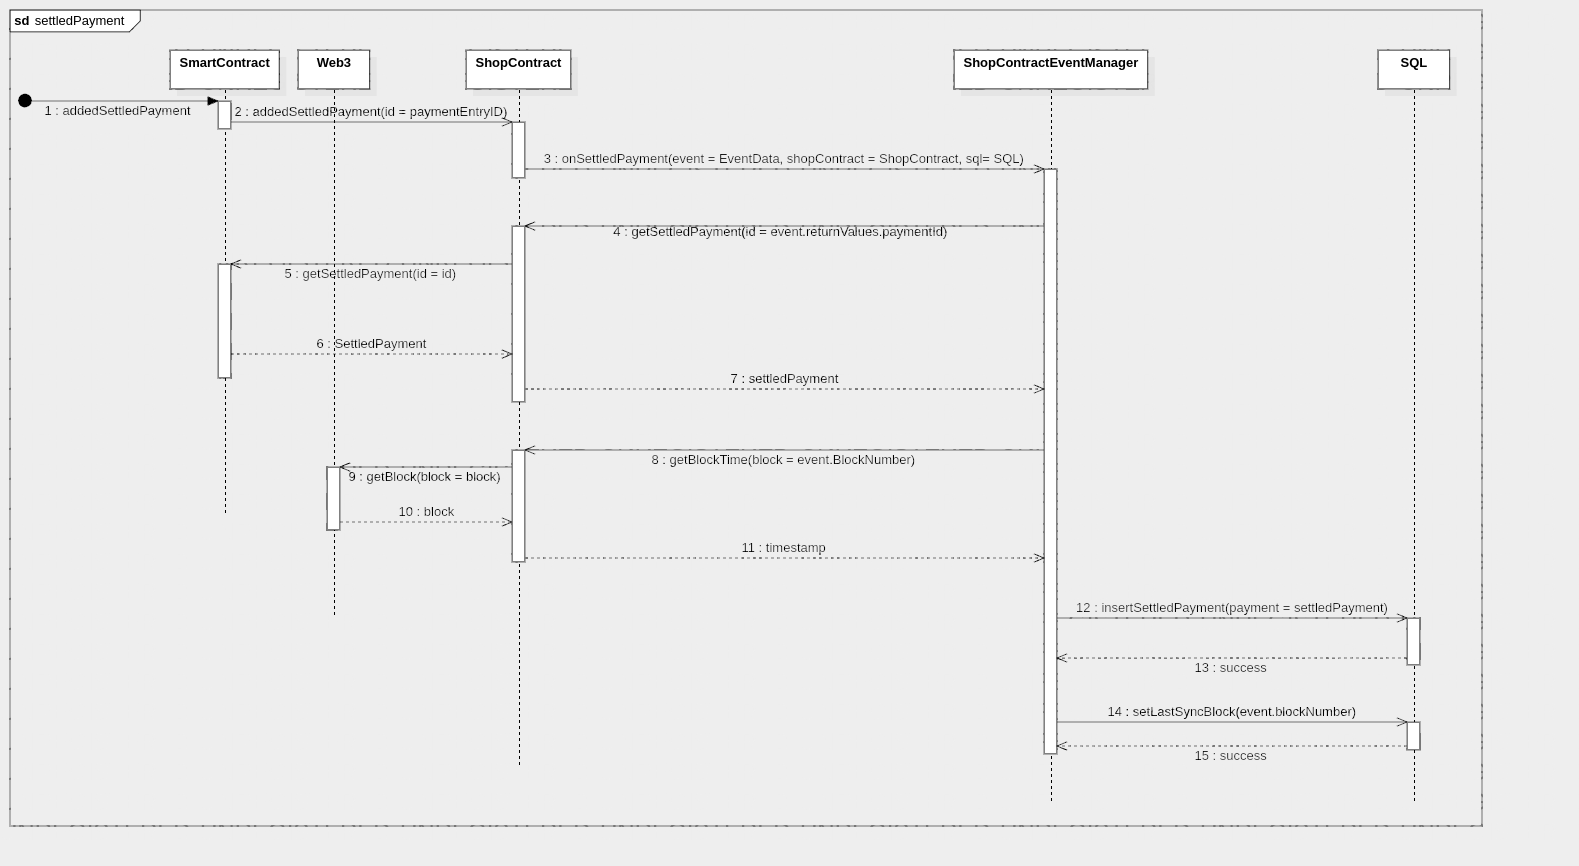
\includegraphics[width=0.85\textwidth]{payment}

\paragraph{Cambio di stato di una transazione}\\
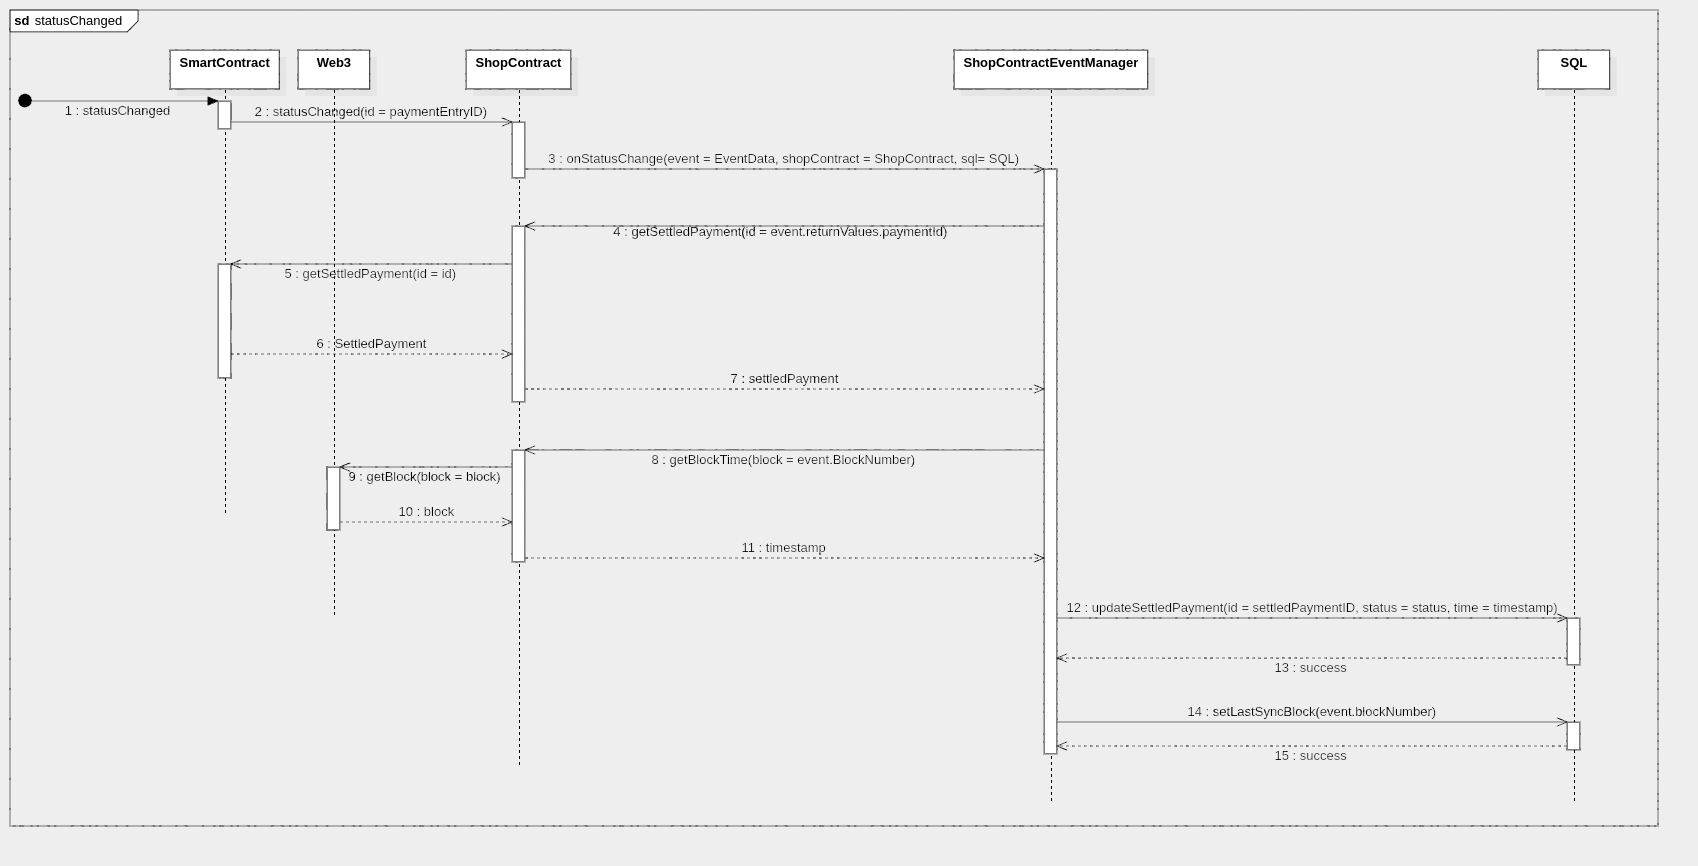
\includegraphics[width=0.85\textwidth]{status}

\paragraph{Home page}\\
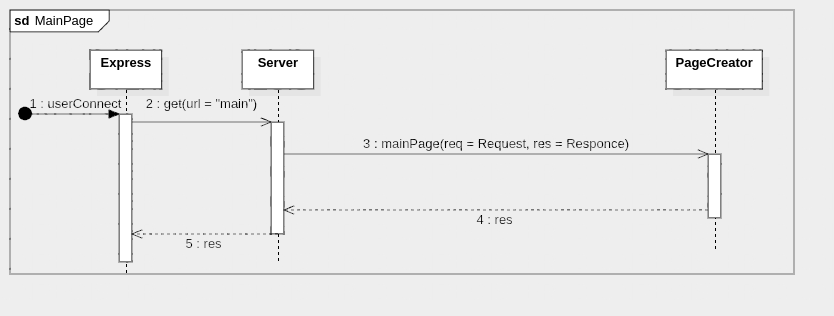
\includegraphics[width=1.0\textwidth]{index}

\paragraph{Landing page di vendita}\\
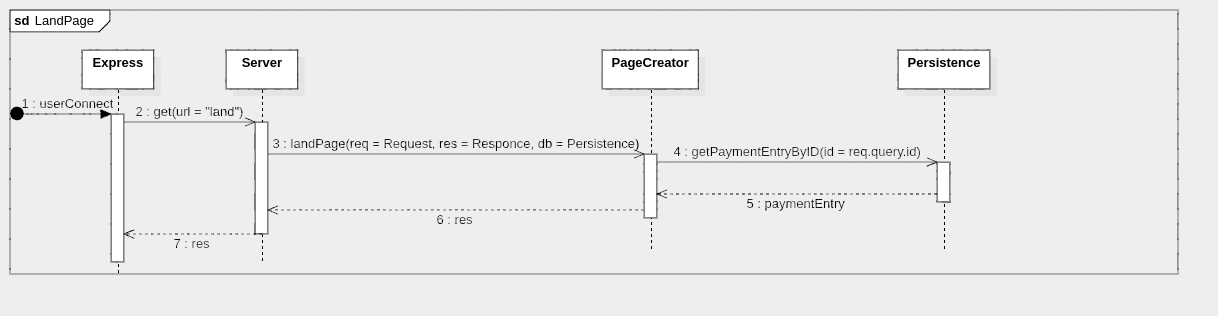
\includegraphics[width=1.0\textwidth]{land}

\paragraph{Dettagli transazione}\\
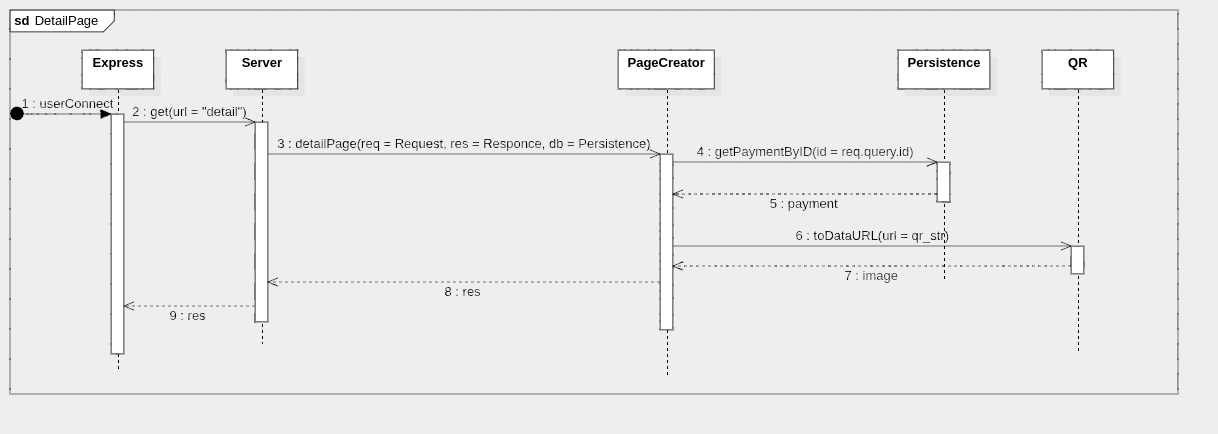
\includegraphics[width=1.0\textwidth]{detail}
\clearpage

\paragraph{Pagina di sblocco fondi (arrivo del pacco)}\\
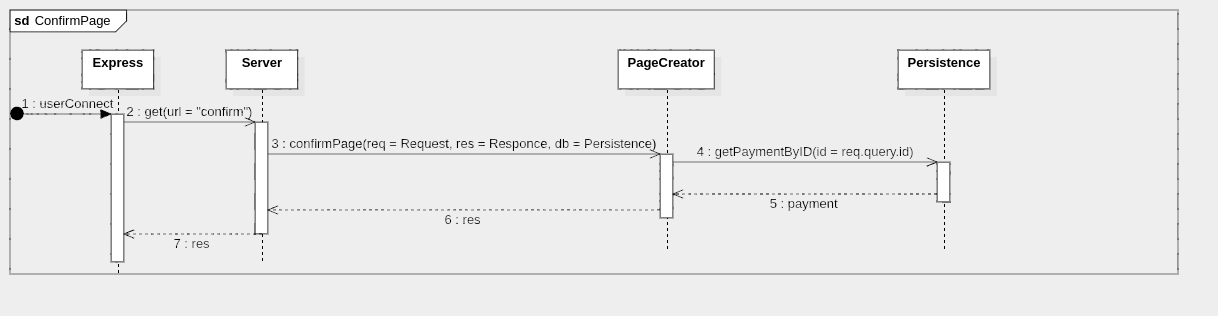
\includegraphics[width=1.0\textwidth]{confirm}

\paragraph{Lista oggetti venduti}\\
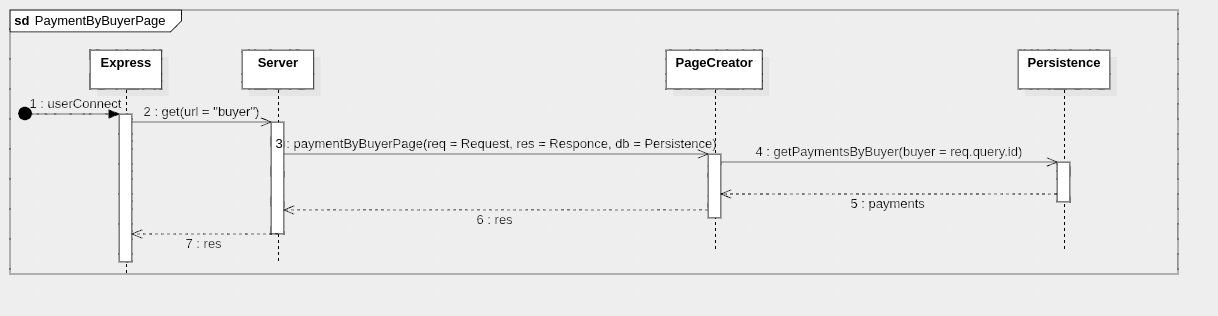
\includegraphics[width=1.0\textwidth]{buyer}

\paragraph{Lista oggetti comprati}\\
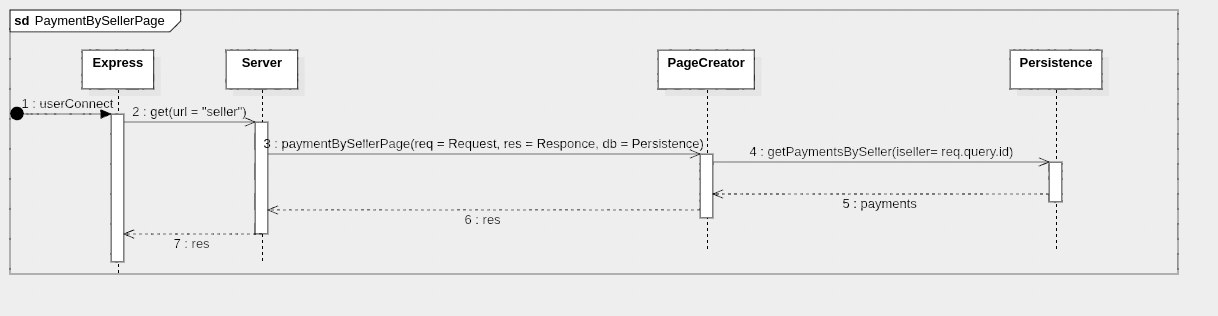
\includegraphics[width=1.0\textwidth]{seller}

\paragraph{Manuale utente}\\
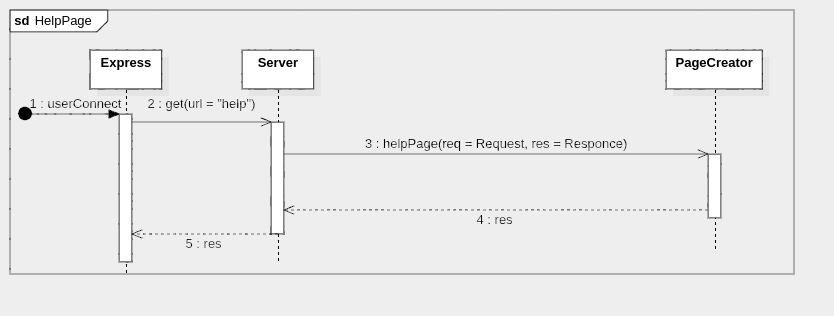
\includegraphics[width=1.0\textwidth]{help}
\end{document}